\documentclass[a4paper]{article}
\def\DOCTITLE{CSC3424 Bio Algorithms}
% Set document attributes
\title{\DOCTITLE}

\usepackage{fullpage}
\usepackage{scrextend}
\usepackage{titlesec}
\usepackage{fancyhdr}
\usepackage{amsmath}
\usepackage{amssymb}
\usepackage[section]{placeins}
\usepackage{booktabs}
\usepackage{hyperref}
\usepackage{tikz}
\usepackage{graphicx}
\usepackage{minted}
\usepackage{subcaption}

% Setup headers and footers
\pagestyle{fancy}
\lhead{}
\chead{\DOCTITLE}
\rhead{}
\rfoot{}
\cfoot{\thepage}
\lfoot{}

% New page for each section
\newcommand{\sectionbreak}{\clearpage}

% Set header and footer sizes
\renewcommand{\headrulewidth}{0.4pt}
\renewcommand{\footrulewidth}{0.4pt}
\setlength{\headheight}{15.2pt}
\setlength{\headsep}{15.2pt}

\setlength{\parskip}{5pt plus 1pt minus 1pt}
\setlength{\parindent}{0pt}

% Newline after paragraph
\newcommand{\Para}[1]{\paragraph{#1}\mbox{}}

% Stuff used in cryptography notes
\newcommand{\Forall}{\;\forall\;}
\newcommand{\Mod}{\: mod \:}

% Stuff used in distributed systems notes
\newcommand{\happenbefore}{\rightarrow}
\newcommand{\orderbefore}{\Rightarrow}
\newcommand{\clockcond}{\leadsto}
\newcommand{\RArrow}{$\rightarrow$}

\def\checkmark{\tikz\fill[scale=0.4](0,.35) -- (.25,0) -- (1,.7) -- (.25,.15) -- cycle;}


\begin{document}

\tableofcontents

\section{Cell and Molecular biology}

\subsection{The Cell}

\begin{itemize}
  \item Minimal unit of life
  \item Cell is a system of many components enclosed in a series of membranes
  \item Small organisms such as fungi and bacteria are unicellular
  \item Plants and animals are generally multicellular
\end{itemize}

\subsubsection{Prokaryotes}

\begin{itemize}
  \item All prokaryotes are single cell
  \item Smaller than eukaryotic cells \\
        ($< 1 \mu \mathrm{m}$ in diameter)
  \item Simple structure \\
        No inner cellular membranes
  \item Very adaptable to environment \\
        Found in almost every habitat
  \item Approximately $5x10^{30}$ prokaryotic cells in the world
  \item Essential for healthy life
\end{itemize}

\Para{Prokaryotic cell}

\begin{itemize}
  \item Less complex than eukaryotic cells
  \item Contain no organelles
  \item Believed to represent the earliest life on earth and that eukaryotic
        cells evolved from prokaryotic cells
\end{itemize}

\begin{figure}[h!]
  \centering
  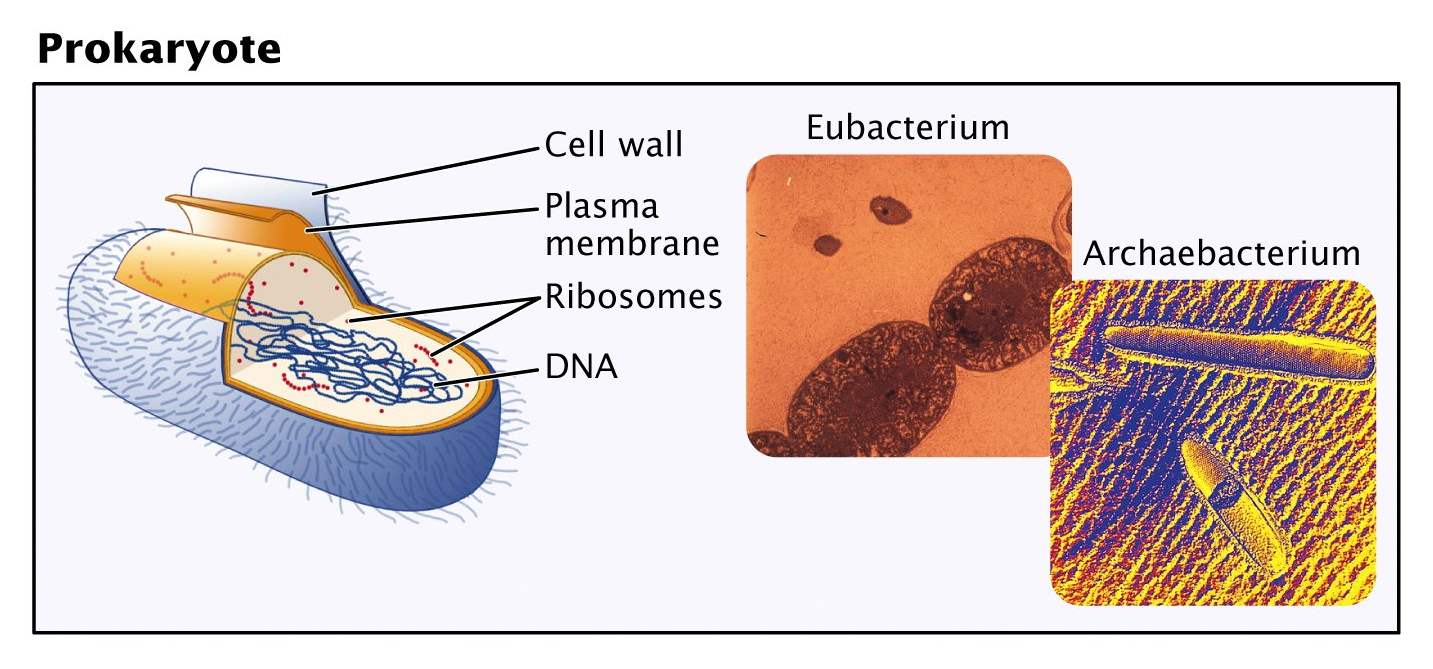
\includegraphics[width=0.7\textwidth]{graphics/prokaryotic_cell.eps}
  \caption{Prokaryotic cell structure}
  \label{fig:prokaryotic_cell}
\end{figure}
\FloatBarrier

\Para{Types of prokaryotes}

Types descend from common ancestor.

\begin{description}
  \item[Eubacteria] \hfill \\
    Common bacteria that affects life daily
  \item[Archaea] \hfill \\
    Tend to exist in extreme habitats (high pressure, temperature, pH)
\end{description}

\subsubsection{Eukaryotes}

\begin{itemize}
  \item More structurally and biochemically complex than prokaryotes
  \item Evolutionarily more recent
  \item Believed to have evolved through endosymbiosis
\end{itemize}

\begin{figure}[h!]
  \centering
  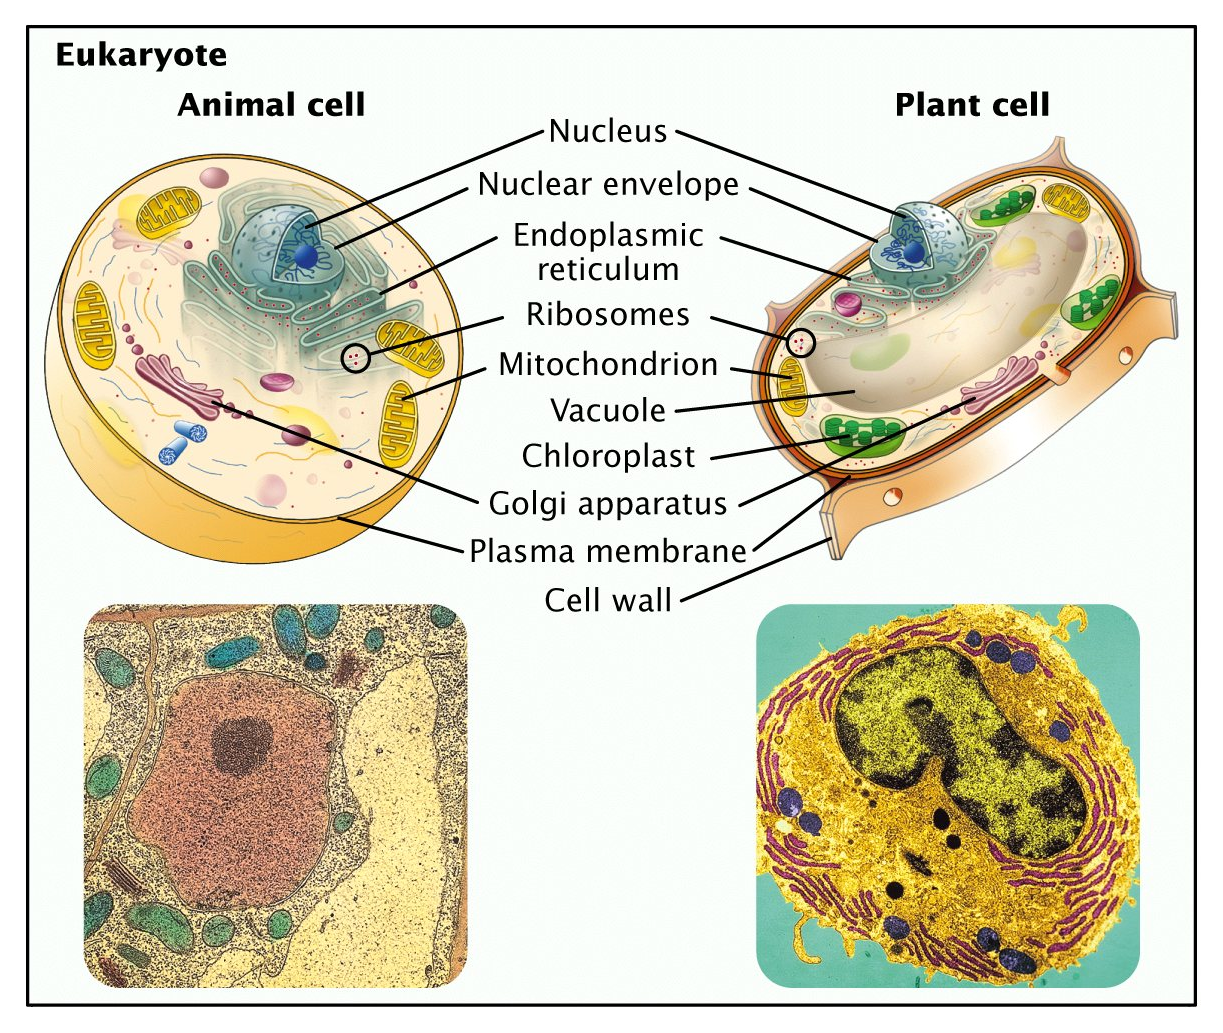
\includegraphics[width=0.7\textwidth]{graphics/eukaryotic_cell.eps}
  \caption{Eukaryotic cell structure}
  \label{fig:eukaryotic_cell}
\end{figure}
\FloatBarrier

\Para{Endosymbiosis}

\begin{itemize}
  \item An ancestral cell engulfed a smaller microbe which continued to survive
        inside it
  \item Both host and prey adapt to new environment and become mutually
        interdependent
\end{itemize}

\subsubsection{Cell functions}

Functions of cells provided by organelle.

\begin{description}
  \item[Nucleus] \hfill \\
    Regulate DNA carrying/replication
  \item[Endoplasmic reticulum] \hfill \\
    System of folded membranes used for transport
  \item[Ribosomes] \hfill \\
    Used to produce proteins
  \item[Mitochondria] \hfill \\
    Provide energy through cellular respiration
  \item[Vacuole] \hfill \\
    Used for storage
  \item[Chloroplasts] \hfill \\
    Used to convert light energy into chemical energy for cell
  \item[Golgi Apparatus] \hfill \\
    Packages and transports proteins
\end{description}

\begin{table}[h!]
  \centering
  \begin{tabular}{@{}lll@{}}
    \toprule
                                & Prokaryotic cells                             & Eukaryotic cells \\
    \midrule
    Nucleus                     & Absent                                        & Present \\
    Cell diameter               & $1-10 \mu \mathrm{m}$                         & $10-100 \mu \mathrm{m}$ \\
    Genome                      & One circular module                           & Multiple linear modules \\
    DNA                         & Not complexed in eubacteria, some in archaea  & Complexed with histomes\\
    DNA quantity                & Small                                         & Large \\
    Membrane-bounded organelles & Absent                                        & Present \\
    Cytoskeleton                & Absent                                        & Present \\
    \bottomrule
  \end{tabular}
  \caption{Comparison of cell types}
  \label{tab:cell_comparison}
\end{table}
\FloatBarrier

\subsubsection{Phenotype from Genotype}

\begin{itemize}
  \item Characteristics of an organism (phenotype) are determined by the
        structure and function of its cells (genotype)
\end{itemize}

\subsection{DNA and genes}

\begin{figure}[h!]
  \centering
  \includegraphics[width=0.2\textwidth]{out/dogma_molecular_biology.eps}
  \caption{Central dogma of molecular biology}
  \label{fig:eukaryotic_cell}
\end{figure}
\FloatBarrier

\subsubsection{Structure of DNA}

\begin{itemize}
  \item Base \\
    Bases bind (A-T, C-G) by Hydrogen bonds
    \begin{itemize}
      \item Pyrimidines
        \begin{itemize}
          \item Cytosine
          \item Thymine
        \end{itemize}
      \item Purines
        \begin{itemize}
          \item Guanine
          \item Adenine
        \end{itemize}
    \end{itemize}
  \item Backbone
    \begin{itemize}
      \item Phosphate \\
        Binds ribose sugar
      \item Ribose sugar \\
        Binds phosphate to base
    \end{itemize}
\end{itemize}

\Para{DNA directionality}

\begin{figure}[h!]
  \centering
  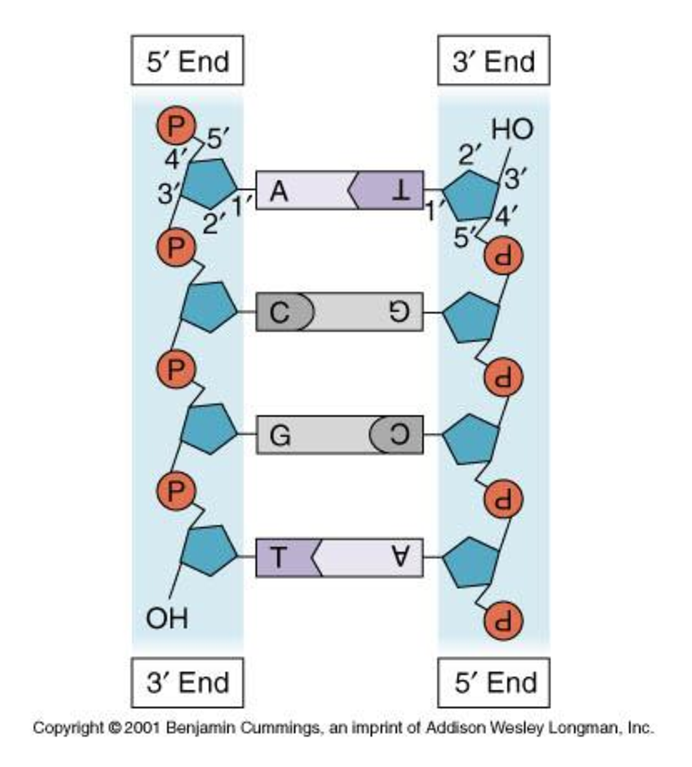
\includegraphics[width=0.4\textwidth]{graphics/dna_directionality.eps}
  \caption{DNA directionality}
  \label{fig:eukaryotic_cell}
\end{figure}
\FloatBarrier

\subsubsection{DNA replication}

\begin{itemize}
  \item Replication is essential for organisms to reproduce
  \item Without replication, cell division could not occur
  \item Replication must be high fidelity but have potential for error (to
        enable evolution)
\end{itemize}

\Para{C-value paradox}

The C-value is the size of an organisms genome (defined as the amount of DNA in
pico grams in a haploid cell).

C-values not reflective of complexity, i.e. no relation between C-value and
number of genes.

\subsubsection{Genome structure}

\Para{Prokaryotic}

\begin{itemize}
  \item Generally small ($<10 \mathrm{M}$ bases)
  \item Single, circular chromosome
  \item Can have plasmids \\
        Disposable genetic elements that often carry genes for antibiotic
        resistance or toxicity
  \item Information dense \\
        Little or no space between genes, genes often overlap
  \item Genes are present in single, uninterrupted units
  \item Multiple genes may be present in single, uninterrupted units
\end{itemize}

\Para{Eukaryotic}

\begin{itemize}
  \item Usually larger than prokaryotic genomes
  \item Multiple, linear chromosomes
  \item Tend to be more information sparse \\
        Large gaps between genes
  \item Genes interrupted by non-coding sequence
    \begin{description}
      \item[Exons] coding
      \item[Introns] non-coding
    \end{description}
\end{itemize}

\subsubsection{DNA packaging}

Nuclear DNA is packaged as chromatin, a structure of DNA, RNA and protein.

Purpose of chromatin:
\begin{itemize}
  \item Packages DNA into a more compact structure
  \item Reinforces macromolecule to allow mitosis
  \item Prevents DNA damage
  \item Regulates gene expression and DNA replication
\end{itemize}

\begin{figure}[h!]
  \centering
  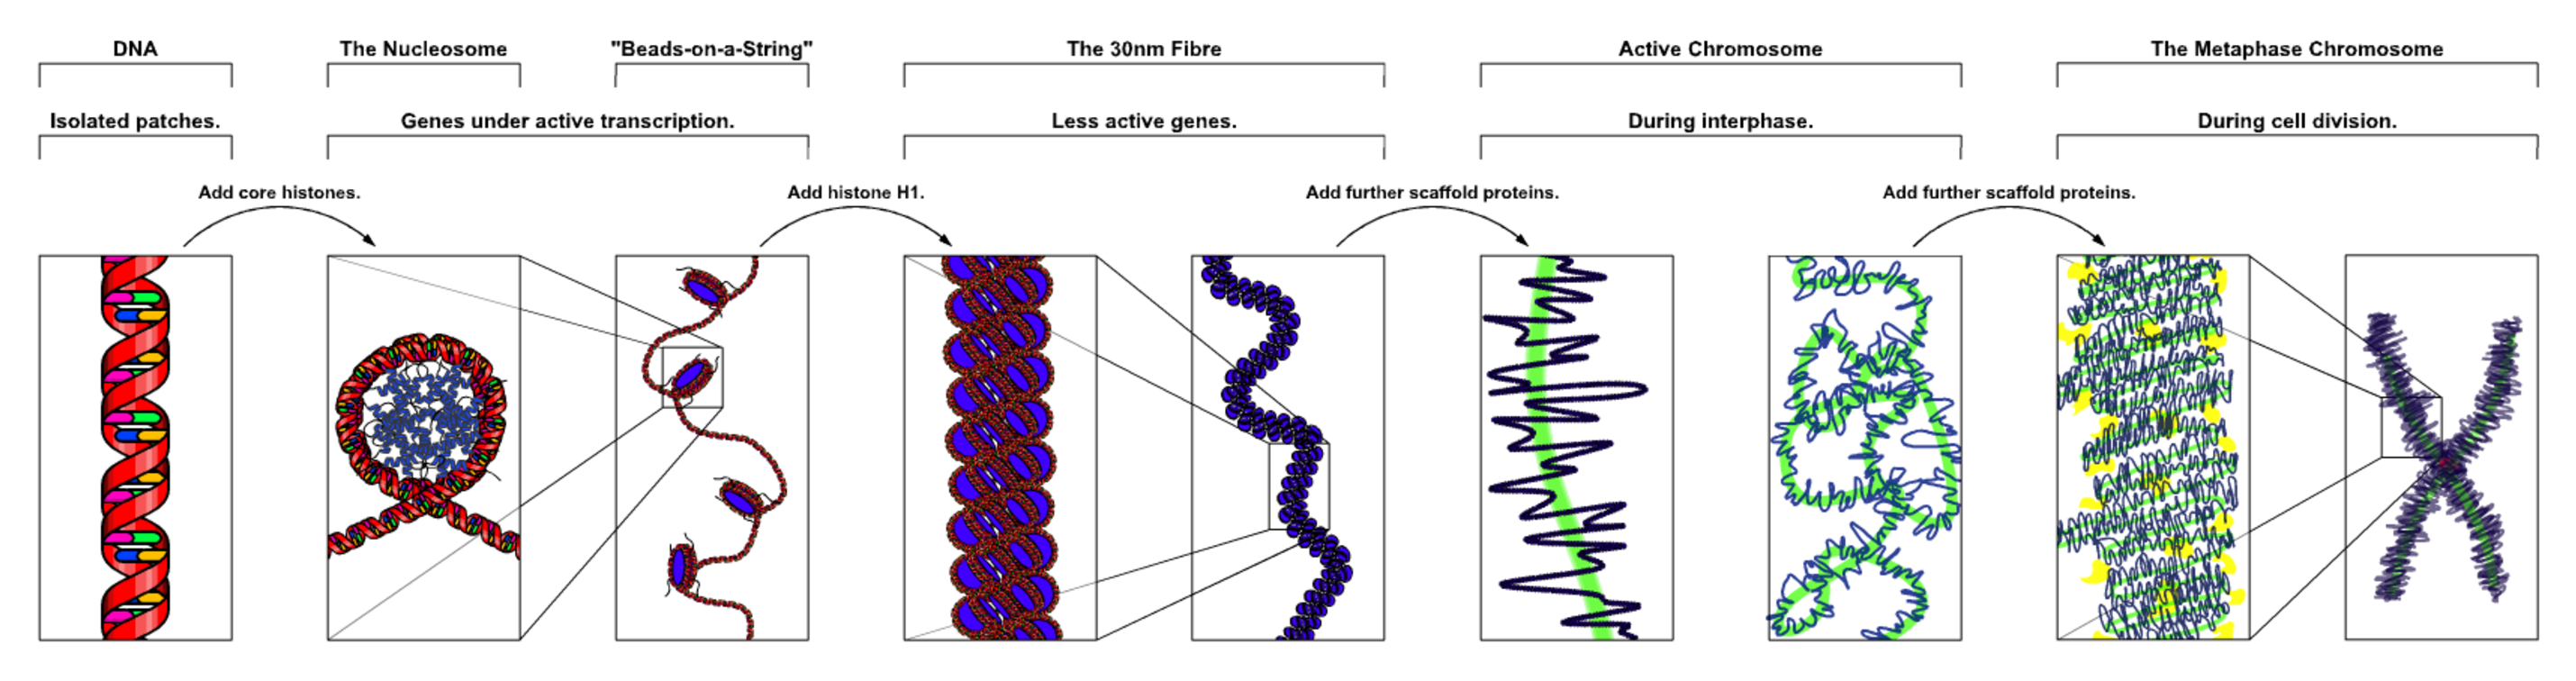
\includegraphics[width=\textwidth]{graphics/chromatin_structures.eps}
  \caption{Chromatin structure}
  \label{fig:chromatin_structures}
\end{figure}
\FloatBarrier

\subsubsection{Manipulating genomes}

\begin{itemize}
  \item Genetic engineering gives multiple techniques for editing the genome of
        an organism
  \item Simplest example is artificial selection to obtain desired traits
  \item Synthetic biology apples engineering principles to biology
\end{itemize}

\subsubsection{Gene structure}

\begin{itemize}
  \item Genes encode functional RNA modules
  \item A gene is a functional part of a chromosome
  \item Every cell contains the same set of genes
\end{itemize}

\subsection{Transcription}

Process of turning information stored in DNA into RNA.

\begin{description}
  \item[Non-template (coding) strand] \hfill \\
    Contains same base sequence as RNA crated
  \item[Template (non-coding) strand] \hfill \\
    Contains anti-codons of RNA
  \item[Promoter] \hfill \\
    Denotes start of RNA coding region
  \item[Coding region] \hfill \\
    RNA coding
  \item[Terminator] \hfill \\
    DNA coding denoting the end of the coding region
\end{description}

\begin{figure}[h!]
  \centering
  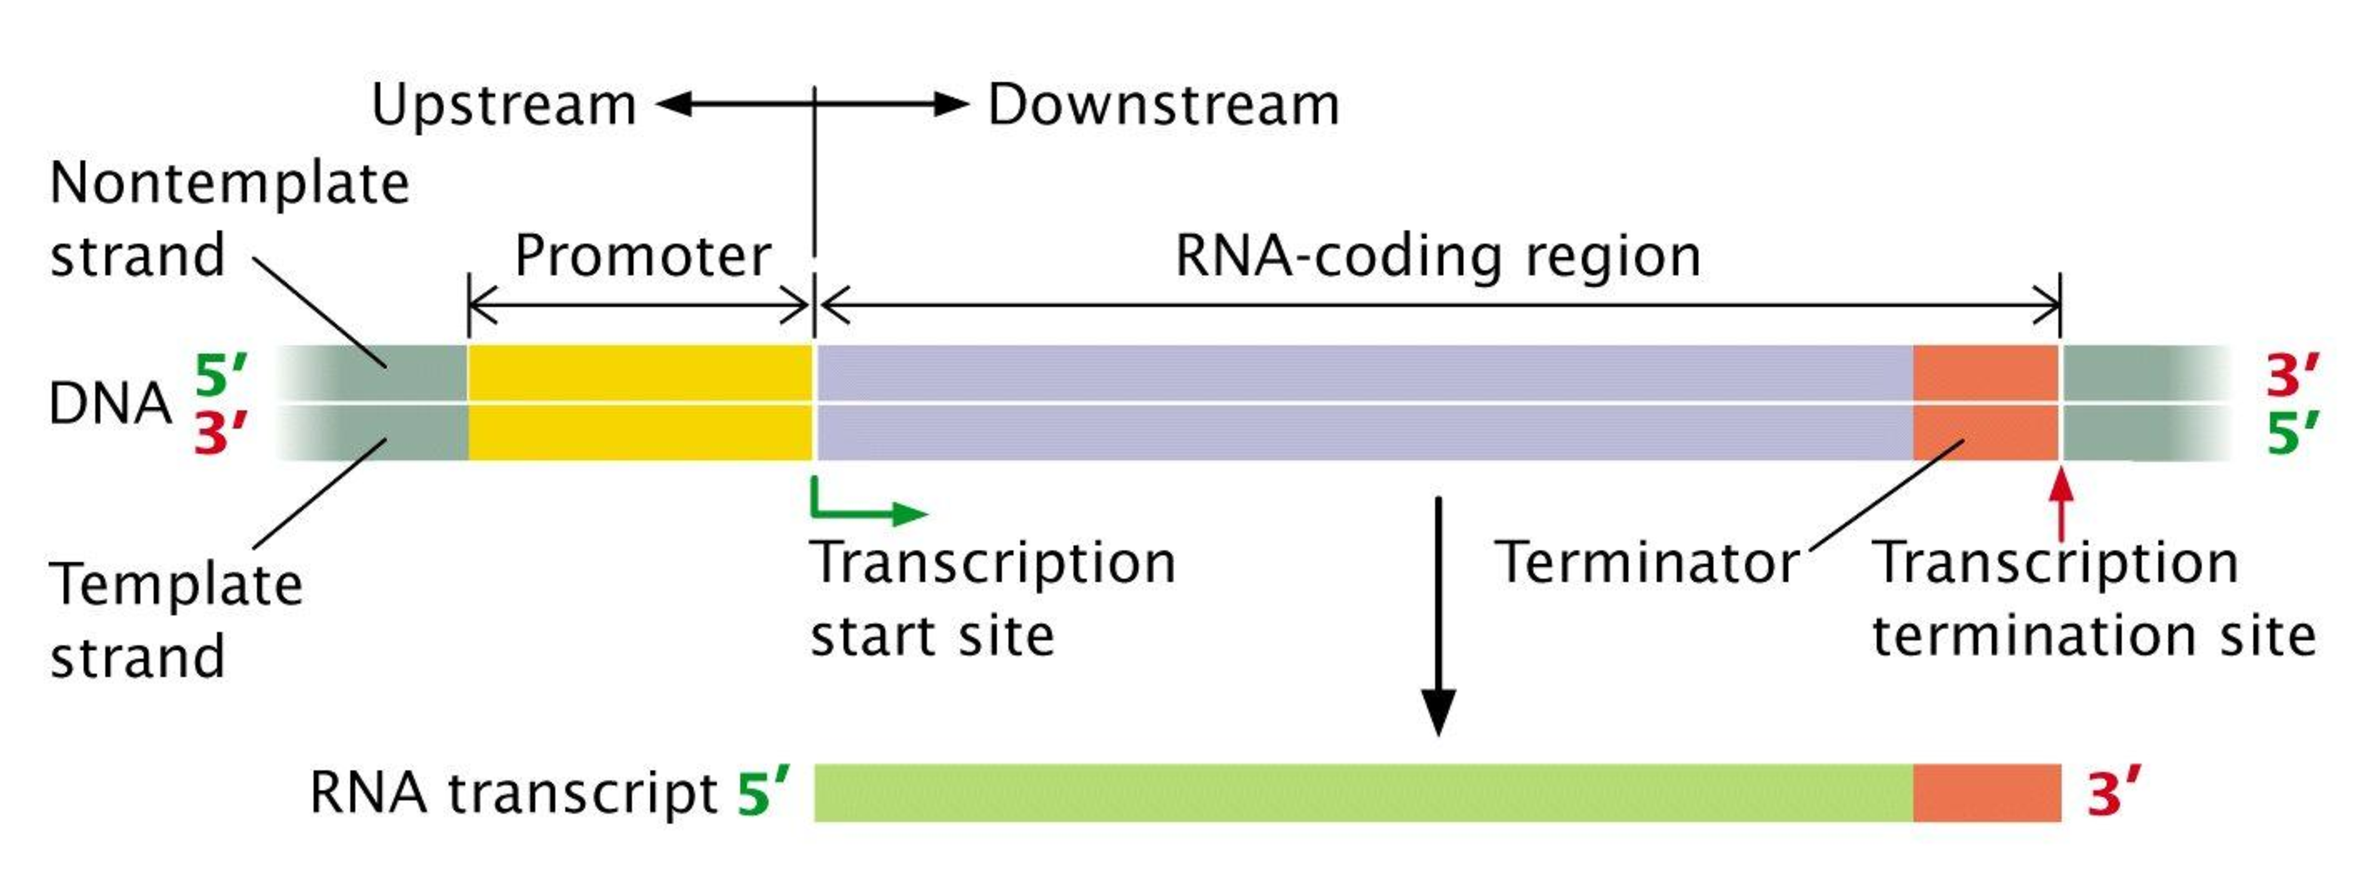
\includegraphics[width=0.8\textwidth]{graphics/dna-rna_transcription.eps}
  \caption{DNA directionality}
  \label{fig:dna-rna_transcription}
\end{figure}
\FloatBarrier

\begin{itemize}
  \item The base Thymine (T) in DNA is replaced with Uracil (U) in RNA
  \item Transcription occurs $5^{\prime}$ to $3^{\prime}$
  \item RNA polymerase is the enzyme responsible for transcription
  \item Transcription in eukaryotes is more complex
\end{itemize}

\subsubsection{Transcript processing}

Primary transcript must be processed into a mature message.

\begin{itemize}
  \item Addition of $5^{\prime}$ cap
    \begin{itemize}
      \item 7-methlyguanosine
      \item Involved in ribosome binding
      \item Protective
    \end{itemize}
  \item $3^{\prime}$ polyadenylation
    \begin{itemize}
      \item Addition of tail of adenosine to mRNA
      \item Required for nuclear export and stability
    \end{itemize}
  \item Splicing
    \begin{itemize}
      \item Primary transcript contains both introns and exons
      \item Introns must be removed
    \end{itemize}
\end{itemize}

\subsection{Translation}

The process of transforming the information contained in mRNA into an amino acid
chain, which is folded into a protein (amino acids joined by peptide bonds).

\begin{itemize}
  \item Proteins may be structural or have an active role (e.g. enzymes)
  \item Protein function sis determined by its amino acid sequence and its three
        dimensional structure
\end{itemize}

\subsubsection{RNA to protein}

Nucleotide sequence is read in groups of three (codon). Codons are consecutive
and non-overlapping.

Each codon corresponds to one of 20 amino acids.

Special cases:
\begin{description}
  \item[AUG]
    Methionine indicates start of frame
  \item[UAA]
    Frame terminator
  \item[UAG]
    Frame terminator
  \item[UGA]
    Frame terminator
\end{description}

\subsubsection{Amino acid structure}

\begin{itemize}
  \item Common structure to all amino acids
  \item Side chain defines properties of amino acid
\end{itemize}

\begin{figure}[h!]
  \centering
  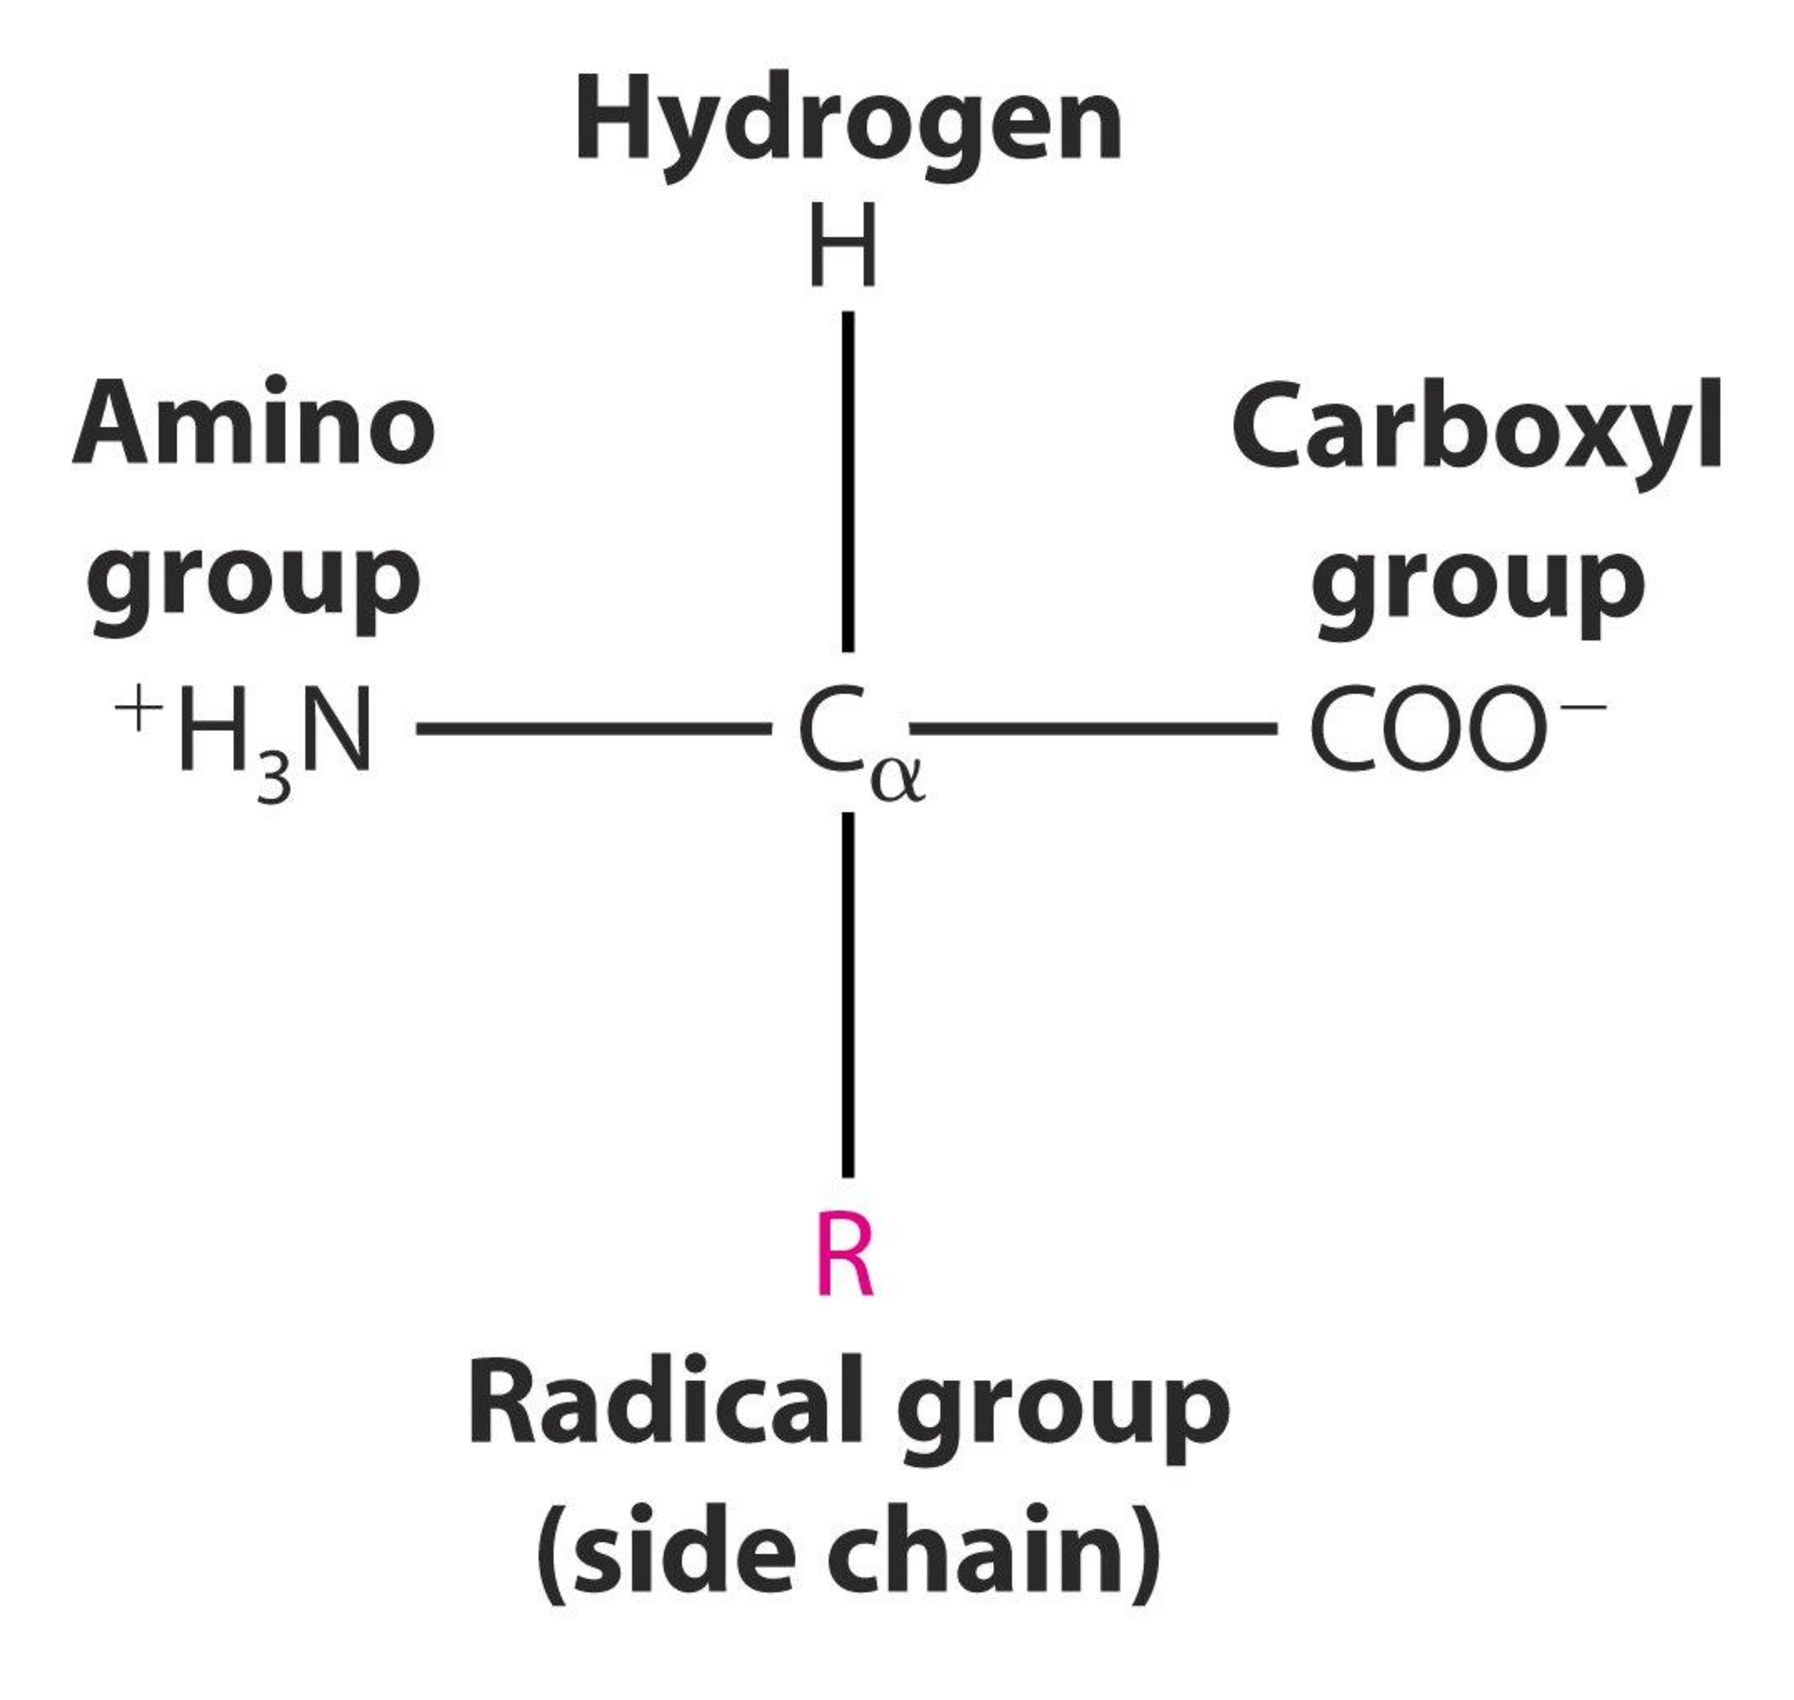
\includegraphics[width=0.35\textwidth]{graphics/amino_acid_structure.eps}
  \caption{Amino acid structure}
  \label{fig:amino_acid_structure}
\end{figure}
\FloatBarrier

Protein is constructed when multiple amino acids are combined into a string by a
peptide bond between the carboxyl group of one acid and the amino group of
another (giving $\mathrm{H}_{2}\mathrm{O}$ as a by-product).

\begin{figure}[h!]
  \centering
  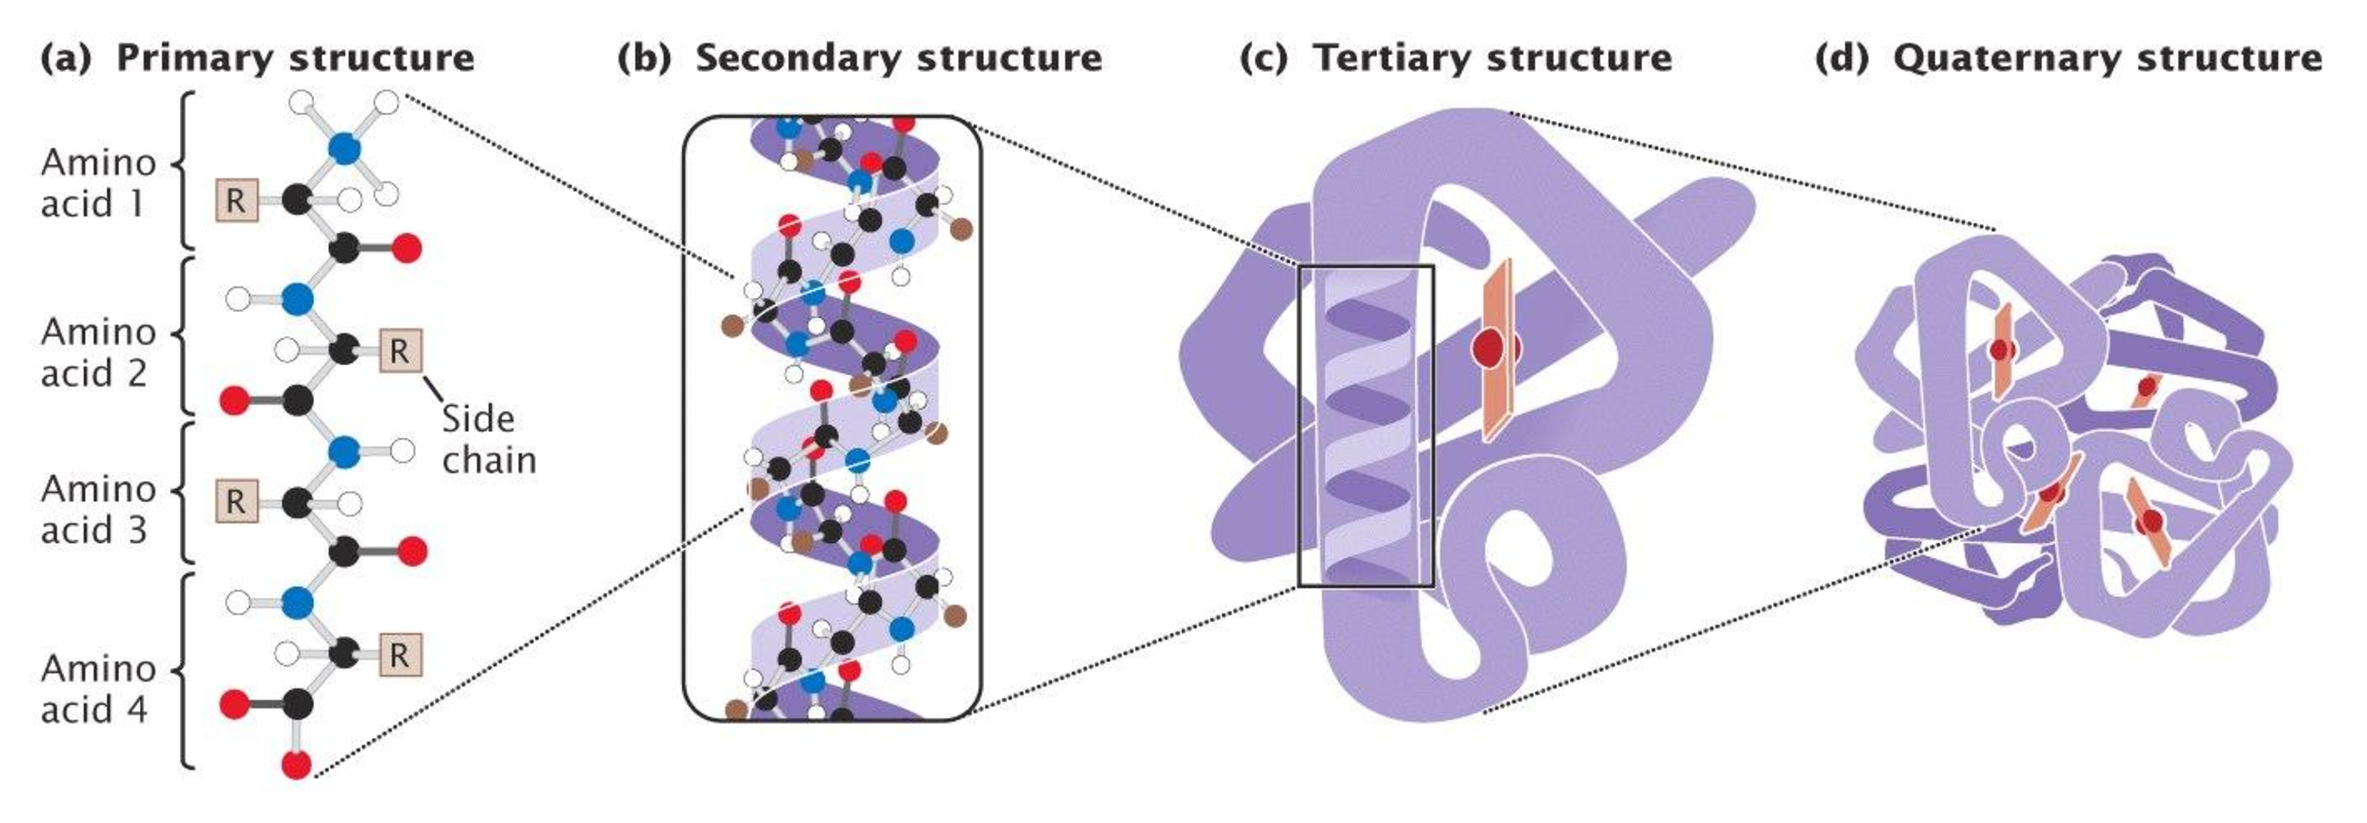
\includegraphics[width=\textwidth]{graphics/protein_structure.eps}
  \caption{Protein structure}
  \label{fig:protein_structure}
\end{figure}
\FloatBarrier

\subsubsection{Ribosomes}

\begin{itemize}
  \item Bind to the region of the mRNA that lies just upstream of the AUG codon
  \item Ribosome Binding Site (RBS) given a consensus sequence which varies with
        organism
\end{itemize}

\subsubsection{Translation process}

\begin{enumerate}
  \item[0] Binding of amino acid to tRNA
  \item[1] Initiation
    \begin{itemize}
      \item Ribosome recognition
        \begin{itemize}
          \item Prokaryotes: mRNA RBS hydrogen bonds with rRNA
          \item Eukaryotes: ribosome attaches to $5^{\prime}$ cap
        \end{itemize}
      \item $\mathrm{tRNA}^{\mathrm{met}}$ binds to AUG codon
    \end{itemize}
  \item[2] Elongation
  \item[3] Termination
    \begin{itemize}
      \item Ribosome pauses at stop codon
      \item Release factor binds
    \end{itemize}
\end{enumerate}

\subsubsection{Control of Gene Expression}

\begin{itemize}
  \item Various levels of control:
    \begin{itemize}
      \item Transcription
      \item Post-transcription
      \item Translation
      \item Post-translation
    \end{itemize}
\end{itemize}

\section{Genome Sequencing, Assembly and Annotation}

\subsection{Sequencing}

Reasons for sequencing:

\begin{itemize}
  \item Identify content and structure
  \item Identify mutations
\end{itemize}

The process of sequencing produces reads. A read is a single continuous sequence
read by the sequencing process.

\subsubsection{Sanger sequencing}

\begin{itemize}
  \item
    Uses DNA polymerase to synthesise DNA

    Enzyme that when given a DNA strand will synthesise the complementary strand

  \item
    A mixture of the polymerase, a primer (small strand of complimentary DNA)
    and deoxynucleotides (DNA nucleotides with fluorescent tag) is made.

  \item
    Products then separated. Multiple methods exist but traditionally using gel
    electrophoresis which allows florescent markers to be seen in four distinct
    "lanes" corresponding to each DNA nucleotide.

  \item
    Accurate but slow

\end{itemize}

\subsubsection{454 pyro-sequencing}

\begin{itemize}
  \item High throughput and lower sample preparation time
\end{itemize}

\subsubsection{Illumina Solexa approach}

\begin{itemize}
  \item Sequencing based on synthesis
  \item Lower cost per sequenced base but high initial cost
\end{itemize}

\subsubsection{Nanopore}

\begin{itemize}
  \item
    Feed DNA through a pore in a surface and detect nucleotides as they pass
    through

  \item
    Faster with minimal sample preparation

\end{itemize}

\subsection{Assembly}

Sequencing produces several fragments of the full genome, in order to obtain the
sequence of the full genome such subsequences must be assembled.

Individual reads are assembled to form contigs. A contig is a group of copied
pieces of DNA representing overlapping regions of a chromosome.

Contigs are assembled to give complete sequences.

\subsubsection{Shotgun sequencing}

\begin{itemize}
  \item
    Long sequences are assembled based on overlaps between several subsequences

  \item
    Region in full sequence should ideally be covered by several subsequences
    to ensure good confidence

    For Sanger sequencing 6 fold redundancy is required

  \item
    Nucleotide at a given position in the final sequence is given by the most
    common nucleotide in the aligned reads/contigs

  \item
    Assembly can be parameterised in terms of number of mismatches between
    aligned reads/contigs allowed at a given point in the final sequence

  \item
    Computationally intensive method: uses naive string searching which becomes
    very slow for large genomes and large number of reads

\end{itemize}

\subsubsection{deBruijn assembly}

\begin{itemize}
  \item
    Split data into a series of small equal length oliomers where oliomers are
    generated by advancing a sliding window along a sequence one nucleotide at a
    time

  \item
    Build a deBruijn graph of all oliomers where edges represent an alignment
    between the two joined oliomers

  \item
    If successful the graph structure will be a single string containing the
    aligned sequence, where the sequence forms an Euclidean path through all
    nodes

  \item
    The choice of the length $k$ of the oliomers is critical to the algorithm
    operating correctly.

    A sub-optimal value of $k$ will cause closed loops in the graph which
    prevents the correct sequence being obtained

\end{itemize}

\subsubsection{Finishing}

After alignment several gaps may be left in the final sequence, leaving the
result as a series of contigs.

Can be caused by lack of experimental data or issues with the wet experiment,
i.e. AT/GC right regions, homopolymenrs, etc.

Ideal solution is to perform more wet experiments.

\subsubsection{Templates}

When assembling the sequence of a new organism with known relatives the genomic
sequence of the relative can be used to assist positioning of the individual
contigs.

This is done by aligning the contigs to the genomic sequence of the relative.

\subsection{Annotation}

Consensus sequences are analysed to discover features details of which are
stored along with the sequence and the region of the sequence it is relevant to.

Typically a time and resource intensive task in the form of a pipeline of
individual tools used to identify specific features.

\subsubsection{Gene finding}

Open reading frames are a region starting with the initialisation codon
(\texttt{ATG}) and ending in one of three stop codons.

Gene finding can be done using one of two main approaches; comparative genomics
or ab initio.

Comparative genomics uses similarity between regions in a sample and other known
samples to infer the structure of a gene.

Ab initio methods are based on determining gene structure based solely on the
experimental data and known biological theories. External data can be used to
improve prediction accuracy.

Prediction of protein coding genes in bacterial genomes is simple and relatively
accurate. In eukaryotes predicting intron-exon regions is only around 65\%
accurate and non-coding exons can cause issues.

\section{Evolution}

Key relevance is similarity between close evolutionary ancestors which aids
prediction of features such as protein function and structure from a sequence.

\subsection{Mutations}

\Para{Point Mutation}

When a single nucleotide in the DNA sequence changes.

This can have several different effects on the protein sequence:

\begin{description}
  \item[Silent] \hfill \\
    The change in DNA sequence does not change the protein sequence.

    e.g. the mutation \texttt{TTC $\rightarrow$ TTT} gives
    \texttt{Lys $\rightarrow$ Lys}

  \item[Nonsense] \hfill \\
    The change in DNA sequence causes a change in protein sequence that does not
    make sense.

    e.g. the mutation \texttt{TTC $\rightarrow$ ATC} gives
    \texttt{Lys $\rightarrow$ STOP}

  \item[Missense] \hfill \\
    The change in DNA sequence causes a change in protein sequence that is valid
    but may affect the function.

    This can be either conservative in which case the new protein has a similar
    function to the previous or non-conservative in which case the functional
    change is significant.

\end{description}

\Para{Deletion}

Where a section of the sequence is removed.

\Para{Duplication}

Where a section of the sequence is duplicated and inserted after the original
section.

\Para{Inversion}

Where a section of the sequence is reversed in the new sequence.

\Para{Insertion}

Where a section of the sequence of one chromosome is inserted into the sequence
of another chromosome.

\Para{Translocation}

Where two sections of the sequence of two different chromosomes are swapped.

\Para{Frameshift mutations}

Mutations where the relative location of coding information is changed due to
the insertion, deletion or exchange of a subsequence of a different length to
the original.

\subsubsection{Gene duplication}

\begin{itemize}
  \item
    Evolutionary constraints define the tolerance of how much the gene can
    diverge from its original function after an evolutionary cycle.

  \item
    After gene duplication duplicates have reduced evolutionary constraints as
    the original copy still exists therefore retention of the original function
    is less important.

  \item
    Gene duplication leads to wider divergence in function and evolution of new
    proteins.

  \item
    In bacteria gene duplication can be triggered by external stimuli.

    e.g. temperature, pressure, starvation, etc.

  \item
    In eukaryotes gene duplication is vital for evolution. Around $\frac{1}{3}$
    of a eukaryotic genome consists of duplicates.

  \item
    Duplicate genes with redundant functions can help towards protection against
    deletion mutations.
\end{itemize}

\subsection{Homology, orthology and parology}

\begin{description}
  \item[Homology] \hfill \\
    Genes that share a common ancestor.

  \item[Orthology] \hfill \\
    Homologous genes which diverged as a result of speciation.

  \item[Parology] \hfill \\
    Homologous genes within the same genome created as a result of gene
    duplication.

  \item[Xenology] \hfill \\
    Homologous genes where one gene has been obtained through transfer of
    genetic material between organisms.

\end{description}

\begin{figure}[h!]
  \centering
  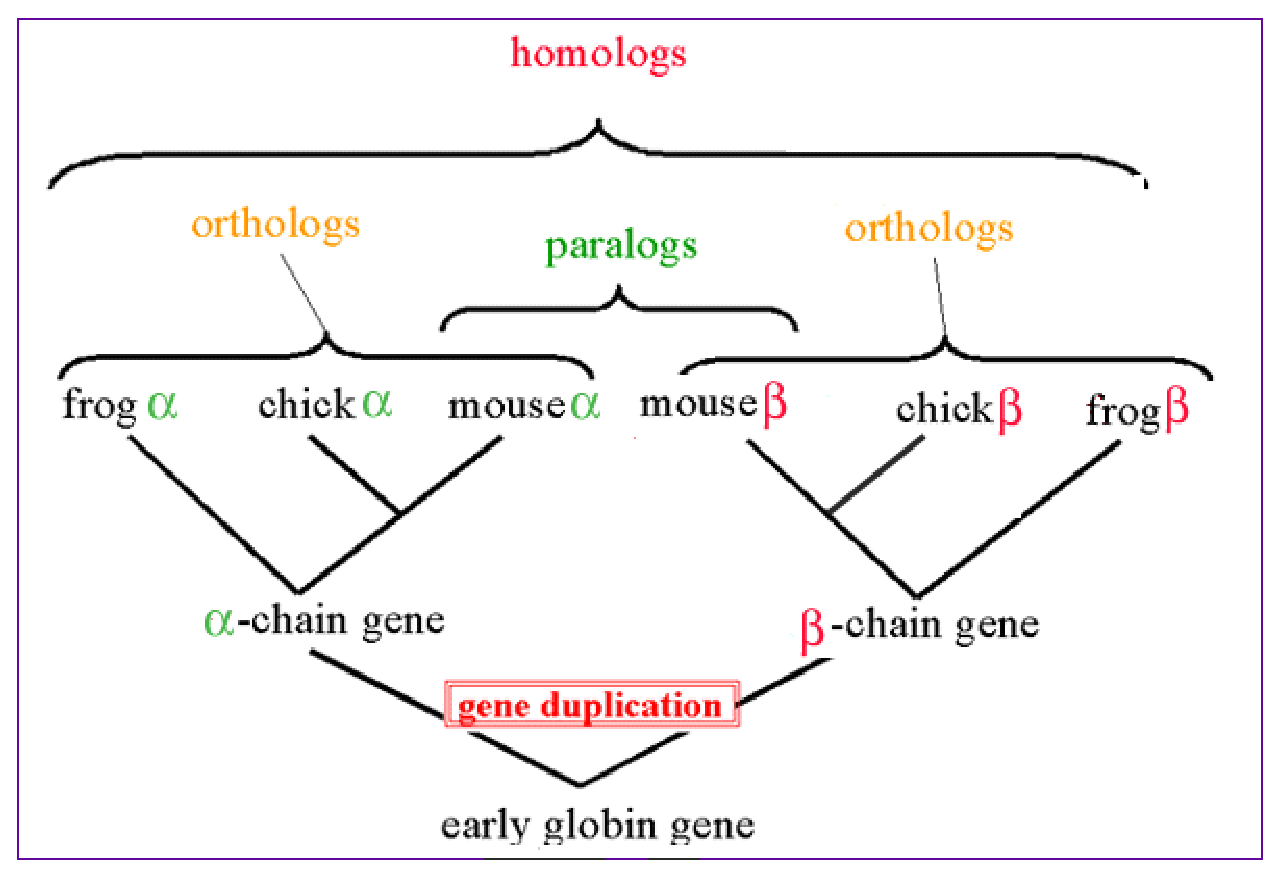
\includegraphics[width=0.7\textwidth]{graphics/homology_orthology_parology.eps}
  \caption{Relationship between homology, orthology and parology}
  \label{fig:homology_orthology_parology}
\end{figure}
\FloatBarrier

\subsection{Homology}

\begin{itemize}
  \item
    Proteins and genes that have diverged from a common ancestor are homologous.

  \item
    Homology is a boolean state, not analogous to sequence similarity.

  \item
    Homology cannot be definitively determined from sequence similarity alone,
    it can however be inferred if the sequences are more than 50\% similar.

  \item
    Homologous proteins often share properties: same/related function, sites,
    structure.

  \item
    As sequences diverge non-conservative mutations increase and the sequence
    similarity to the common ancestor decreases while remaining functionally
    similar, this can make determining homology difficult.
\end{itemize}

\subsection{Orthology}

\begin{itemize}
  \item
    Homologous genes from different genomes within the same gene family.

  \item
    Derived as a result of speciation.

  \item
    Often encode proteins that perform the same function in different organisms.
\end{itemize}

\subsection{Parology}

\begin{itemize}
  \item
    Homologous genes within the same genome within different gene families.

  \item
    May perform different functions in each host due to functional change with
    evolution.
\end{itemize}

\section{Phylogenetics}

\begin{itemize}
  \item
    The study of evolutionary relationships between groups of organisms.

  \item
    Produces hypothesis about evolutionary history of organisms.

  \item
    Species (genes) typically shows as evolving as per a tree structure.

  \item
    Based on inferring information about evolutionary history from present day
    knowledge.

    Phylogenetics are hypotheses.

    Changes as new data becomes available.

  \item
    Can use molecular data to infer phylogenetic relationships.
\end{itemize}

\subsection{Workflow}

\subsubsection{Obtain sequences}

\begin{itemize}
  \item
    Selection of sequences is dependant on the research.

  \item
    Typically use well conserved genes.
\end{itemize}

\subsubsection{Alignment}

\begin{itemize}
  \item
    TODO
\end{itemize}

\subsubsection{Masking}

\begin{itemize}
  \item
    Separate areas of high similarity from those of low similarity.

  \item
    Areas of high similarity infer homology, low similarity cannot be used to
    infer either way.
\end{itemize}

\subsubsection{Evolutionary model fitting}

Multiple methods:

\begin{itemize}
  \item
    Unweighted pair group method with arithmetic mean (UPGMA) (simple)

  \item
    Maximum likelihood (advanced)

  \item
    Bayesian (advanced)
\end{itemize}

\Para{Unweighted pair group method with arithmetic mean}

\begin{itemize}
  \item
    Uses distance matrix that tabulates the distance between each pair of
    species.

  \item
    Each iteration merge two closest species and recalculate matrix values based
    on mean of merged species.

  \item
    Repeat until all species are grouped.

  \item
    Order of grouping gives tree structure.
\end{itemize}

Example with 5 species: \texttt{A}, \texttt{B}, \texttt{C}, \texttt{D},
\texttt{E}.

\begin{table}[h!]
  \centering
  \begin{tabular}{@{}lllll@{}}
    \toprule
    Species & A  & B  & C  & D \\
    \midrule
    B       & 9  & -  & -  & - \\
    C       & 8  & 11 & -  & - \\
    D       & 12 & 15 & 10 & - \\
    E       & 15 & 18 & 13 & 5 \\
    \bottomrule
  \end{tabular}
  \caption{UPGMA iteration 1}
  \label{tab:upgma_1}
\end{table}
\FloatBarrier

Merge \texttt{D} and \texttt{E} (shortest distance 5):

\begin{table}[h!]
  \centering
  \begin{tabular}{@{}llll@{}}
    \toprule
    Species & A    & B    & C    \\
    \midrule
    B       & 9    & -    & -    \\
    C       & 8    & 11   & -    \\
    DE      & 13.5 & 16.5 & 11.5 \\
    \bottomrule
  \end{tabular}
  \caption{UPGMA iteration 2}
  \label{tab:upgma_2}
\end{table}
\FloatBarrier

Merge \texttt{A} and \texttt{C} (shortest distance 8):

\begin{table}[h!]
  \centering
  \begin{tabular}{@{}lll@{}}
    \toprule
    Species & B    & AC   \\
    \midrule
    AC      & 10   & -    \\
    DE      & 16.5 & 12.5 \\
    \bottomrule
  \end{tabular}
  \caption{UPGMA iteration 3}
  \label{tab:upgma_3}
\end{table}
\FloatBarrier

Reconstruct tree from order of merges:

\begin{figure}[h!]
  \centering
  \includegraphics[width=0.4\textwidth]{out/upgma_tree.eps}
  \caption{Phylogenetic tree created using UPGMA}
  \label{fig:upgma_tree}
\end{figure}
\FloatBarrier

\subsubsection{Analyse tree}

\begin{itemize}
  \item
    Tips correspond to modern species.

  \item
    Position of fork in tree in terms of depth is reflective of the point in
    history that the two organisms diverged.
\end{itemize}

\section{Sequence Similarity and Comparison}

\begin{itemize}
  \item Similarity score required for sequence alignment
\end{itemize}

\subsection{String based similarity}

\begin{itemize}
  \item Typically not used for biological sequences
  \item Certain changes are more likely to occur as a result of evolution
\end{itemize}

\subsubsection{Hamming distance}

\begin{itemize}
  \item Number of positions with mismatching characters in two strings of equal
        length
  \item Lower score denotes similar sequences
\end{itemize}

\subsubsection{Levenshtein distance}

\begin{itemize}
  \item Minimum number of edits to change one string into another
  \item Lower score denotes similar sequences
  \item A change can be an addition, deletion or substitution
\end{itemize}

\subsection{Sequence Similarity}

\begin{itemize}
  \item Assignment of variable weights to each misalignment
  \item Additive step scores
  \item Gap penalty for areas of no alignment
\end{itemize}

\Para{DNA and RNA}

\begin{itemize}
  \item
    Typically +1 for match and -1 for mismatch

  \item
    Complex schemes may take into account that a purine-purine or
    pyrimidine-pyrimidine mismatch is more common that a purine-pyrimidine
    mismatch
\end{itemize}

\Para{Proteins}

\begin{itemize}
  \item
    Learn a matrix of scores based on known amino acid changes during evolution

  \item
    Scores derived from frequency of of amino acid substitutions

  \item
    Data encoded in PAM matrices
\end{itemize}

\subsubsection{Gap penalty}

\begin{itemize}
  \item
    Penalise gaps in sequence alignment

  \item
    Larger penalty added for opening a gap than extending an already open gap

  \item
    Typical penalties for DNA:

    \begin{description}
      \item[Opening] 10
      \item[Extending] 0.1
    \end{description}

  \item
    Typical penalties for proteins:

    \begin{description}
      \item[Opening] 11
      \item[Extending] 1
    \end{description}
\end{itemize}

\subsubsection{Percent Accepted Mutation (PAM) matrices}

\begin{itemize}
  \item
    Based on knowledge of evolution

  \item
    Probability of a given change can be determined from alignment of homologous
    sequences

  \item
    Relative frequencies of amino acid changes are encoded in the PAM scoring
    matrix as the probability of mutation to every other amino acid

  \item
    Sample data is restricted to sequences sufficiently similar to ensure
    multiple substitutions have not occurred on the same site

  \item
    A PAM matrix measures sequence divergence

    i.e. a 1 PAM substitution matrix is generated from two sequences that are
    99\% similar

  \item
    To assert similarity of more diverse sequences need matrices for much lower
    sequence similarity

  \item
    Can derive PAM matrices for lower similarity by taking powers of existing
    matrices

  \item
    A range of PAM matrices have been generated in this way and the divergence
    percentage is used in the name of the matrix (e.g. PAM250 denotes expected
    change of 250\%)

  \item
    For use in protein comparison the PAM matrix is first normalised and the
    logarithm taken (known as a log-odds matrix)

    This allows the scores to be added rather than multiplied (as would have had
    to be done with probabilities)
\end{itemize}

\subsubsection{BLOSSUM matrices}

\begin{itemize}
  \item
    Multiple alignments of short, continuous (without gaps) sequences are
    arranged into blocks

  \item
    Substitution frequencies for all pairs of amino acids are calculated for
    each block

  \item
    Used in a similar way to PAM matrices to create log-odds scores for amino
    acid substitution

  \item
    Similarity of protein sequences in a block can be adjusted to obtain
    different similarity matrices

  \item
    All BLOSSUM matrices are derived from direct measurements

    i.e. not extrapolated as is done for PAM

  \item
    BLOSSUM allows for detection of more distantly related sequences than PAM
    by reducing the importance of more similar sequences in the block when
    building the matrix

  \item
    BLOSSUM62 (default for many comparison tools) created from blocks where 62\%
    of the amino acids were identical
\end{itemize}

\subsection{Sequence Alignment}

\begin{itemize}
  \item
    Aligning sequences is useful to determine how similar they are

  \item
    Alignment also shows which parts of the sequence are similar

  \item
    If two proteins have over 45\% identical residue structure then they are
    likely to have a common or related structure

  \item
    If they have over 25\% identical residues then they are likely to have
    similar folding patterns
\end{itemize}

\subsubsection{Exact vs. heuristic}

\begin{itemize}
  \item
    Exact

    \begin{itemize}
      \item
        Guaranteed to find an optimal solution

      \item
        Computationally intensive

      \item
        Good for small numbers of sequences or when algorithm is implemented in
        hardware
    \end{itemize}

  \item
    Heuristic

    \begin{itemize}
      \item
        Not guaranteed to find an optimal solution

      \item
        More computationally efficient

      \item
        Better for searching large databases
    \end{itemize}
\end{itemize}

\subsubsection{Global alignment}

\begin{itemize}
  \item
    Attempts to align all residues in sequence

  \item
    Useful when sequences are very similar and of equal length
\end{itemize}

\Para{Exact method: Trajectories}

\begin{itemize}
  \item
    Trajectory visualised by a 2D matrix with each sequence as indexing row and
    columns

  \item
    Diagonal arrow denotes an alignment between residues

    This can be either a match or mismatch

  \item
    A horizontal arrow denotes a gap in the sequence indexing the columns

  \item
    A vertical arrow denotes a gap in the sequence indexing the rows
\end{itemize}

\begin{figure}[h!]
  \centering
  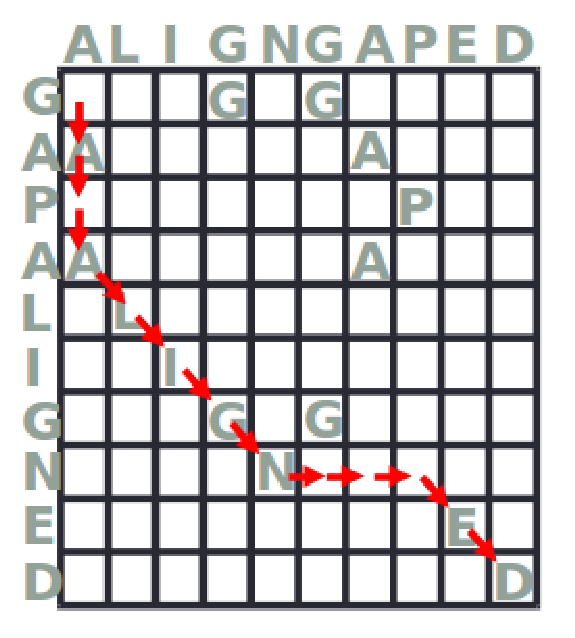
\includegraphics[width=0.3\textwidth]{graphics/alignment_trajectory.eps}
  \caption{Trajectory example}
  \label{fig:alignment_trajectory}
\end{figure}
\FloatBarrier

\Para{Global alignment: Needleman Wunsch algorithm}

\begin{itemize}
  \item
    Computationally intensive

  \item
    Can use PAM, BLOSSUM, etc. as a similarity matrix to obtain alignment score

  \item
    Construct matrix of dimensions $(m, n)$ where $m$ and $n$ are the sizes of
    each sequence

  \item
    A cell in the matrix $(i, j)$ will contain the optimal score of aligning the
    first $i$ residues of the first sequence with the first $j$ residues of the
    second

  \item
    Matrix is filled incrementally

  \item
    The value of cell $(i, j)$ is determined by the value of cells $(i-1, j)$,
    $(i, j-1)$ and $(i-1, j-1)$

    The value is the lowest movement score given by the score of the last cell
    plus the score of the alignment of the current cell (i.e. score of mismatch,
    gap opening or gap extending)

  \item
    An arrow is placed from the cell in the direction of the lowest score

  \item
    When all cells are filled cell $(m, n)$ will contain the optimal score of
    the global alignment

  \item
    By following the arrows from cell $(m, n)$ one can obtain the optimal global
    alignment(s)

    Note that multiple equally scored optimal alignments may be possible, each
    indicated by branching and joining in the path
\end{itemize}

Example:

\begin{figure}[h!]
  \centering
  % 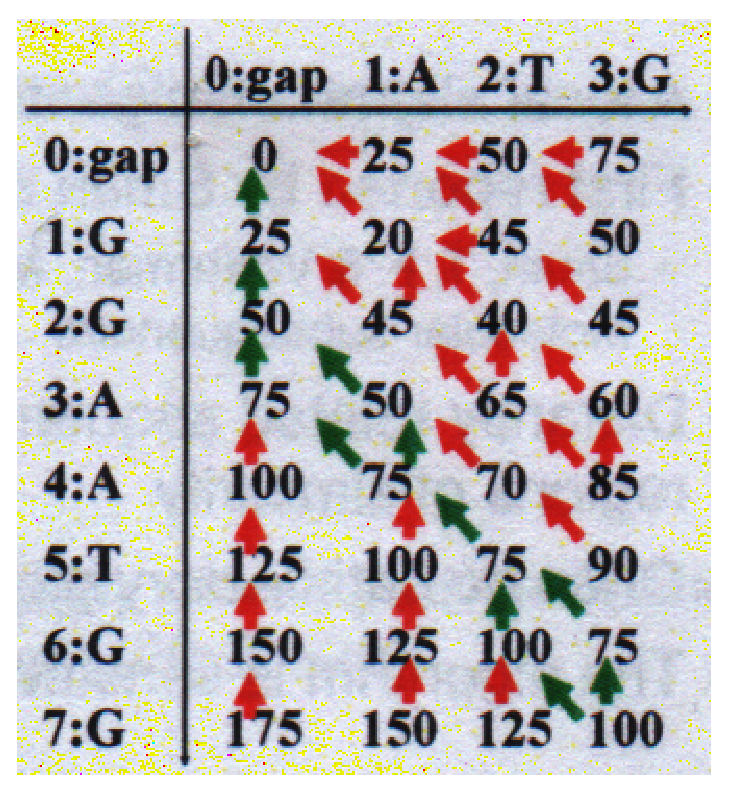
\includegraphics[width=0.7\textwidth]{graphics/nw_alignment_eg.eps}
  TODO
  \caption{Needleman Wunsch alignment example}
  \label{fig:nw_alignment_eg}
\end{figure}
\FloatBarrier

Four optimal alignments for figure \ref{fig:nw_alignment_eg}:

\begin{itemize}
  \item
    \texttt{ggaatgg}

    \texttt{---atg-}

  \item
    \texttt{ggaatgg}

    \texttt{---at-g}

  \item
    \texttt{ggaatgg}

    \texttt{--a-t-g}

  \item
    \texttt{ggaatgg}

    \texttt{--a-tg-}
\end{itemize}

\subsubsection{Local alignment}

\begin{itemize}
  \item
    Aligns subsection of sequences that align best

  \item
    Useful when sequences contain sub regions of similarity
\end{itemize}

\Para{Local alignment: Smith Waterman algorithm}

\begin{itemize}
  \item
    Variation of global alignment method using matrix

  \item
    At initialisation all cells are set to zero

  \item
    Gaps at the beginning of the sequence are not penalised

  \item
    The additional option of ending the sequence is also considered when
    deciding the score of a given cell

  \item
    The optimal score (end of the alignment) can appear anywhere in the matrix

  \item
    The start of the alignment can appear anywhere before the end of the
    alignment in the matrix
\end{itemize}

Example:

\begin{figure}[h!]
  \centering
  % 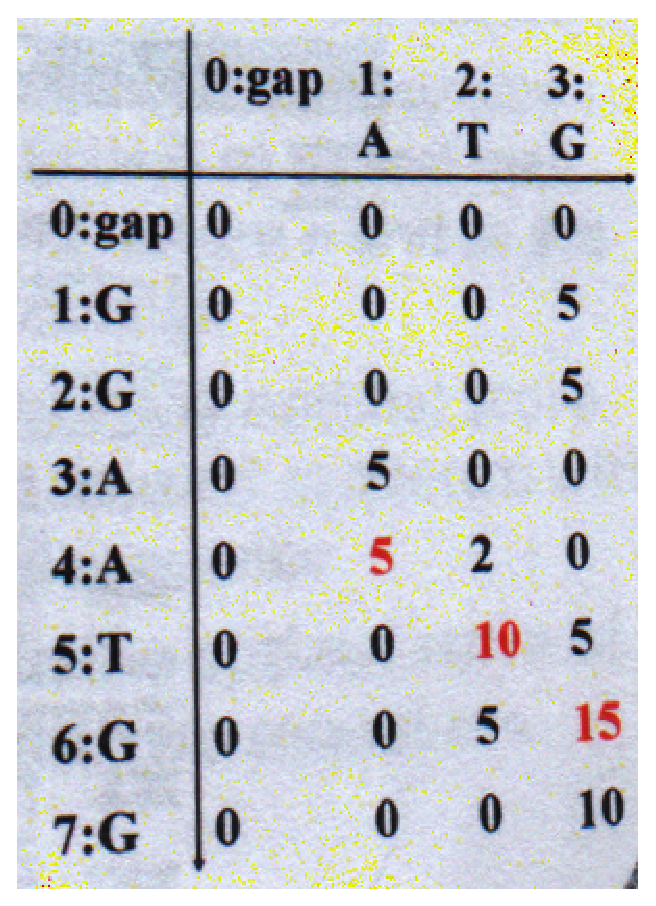
\includegraphics[width=0.7\textwidth]{graphics/sw_alignment_eg.eps}
  TODO
  \caption{Smith Waterman alignment example}
  \label{fig:sw_alignment_eg}
\end{figure}
\FloatBarrier

Scores are given by:

\begin{itemize}
  \item Match = +5
  \item Mismatch = -3
  \item Gap = -5
\end{itemize}

Value of cell $(i, j)$ is given by:

\[
  S(i, j) = max
    \left (
    \begin{array}{ll}
      S(i-1, j-1) + mis/match score \\
      S(i-1, j) + gap score \\
      S(i, j-1) + gap score \\
      0 \\
    \end{array}
    \right )
\]

Where 0 ends the alignment.

\Para{Approximate method: k-tuple}

\begin{itemize}
  \item
    Take a sample sequence and split it into all possible incremental
    subsequences of a given size $k$

    For proteins: $k = 3$

  \item
    Search a database for each substring

    Reduces number of candidate strings

  \item
    Then extend alignment using sequences of good alignment with substrings
\end{itemize}

\Para{BLAST algorithm}

\begin{itemize}
  \item
    (Basic Local Alignment Search Tool)

  \item
    ~100 times faster than exact dynamic programming approaches
\end{itemize}

Workflow:

\begin{enumerate}
  \item[1]
    Split into $k$ letter substrings.

    e.g:
    \texttt{\hfill \\
      MATCHES \\
      MAT.... \\
      .ATC... \\
      ..TCH.. \\
      ...CHE. \\
      ....HES \\
    }

  \item[2]
    Align each sequence to all possible $k$ length subsequences

  \item[3]
    Compute the similarity scores of all alignments

    \begin{itemize}
      \item
        Discard those that have a score less than the neighbourhood score
        threshold

      \item
        This greatly reduces the number of alignments to be considered
    \end{itemize}

  \item[4]
    Search database for exact matches of each word

  \item[5]
    Ungapped alignments

    \begin{itemize}
      \item
        If for the same sequence in the database, two non-overlapping hits are
        found less than a threshold number of residues apart

      \item
        In this case the alignment is extended starting with these hits as long
        as the score is no worse than a given threshold respective of the best
        score found so far
    \end{itemize}

  \item[6]
    Gapped alignments

    \begin{itemize}
      \item
        Dynamic programming method is used for gapped alignments
    \end{itemize}
\end{enumerate}

\Para{E value}

\begin{itemize}
  \item
    Describes the number of hits expected when searching a database of a given
    size

  \item
    Decreases exponentially as the score increases

  \item
    Essentially describes the amount of background noise

    e.g. $E=1$ denotes that in a database of the current size, it is expected to
    find 1 match with a similar score by chance

  \item
    Lower E value denotes a higher probability that the sample sequence has
    matched a homologous protein

    However, almost identical short alignments have a high E value as the length
    of the sequence is taken into account
\end{itemize}

\subsection{Multiple Sequence Alignment}

\begin{itemize}
  \item
    Multiple sequences laid out in a grid such that:

    \begin{itemize}
      \item
        Relative positions of residues within any one sequence is conserved

      \item
        Similar residues in all sequences are brought into the same vertical
        register
    \end{itemize}

  \item
    Exact approach is too computationally expensive to use

  \item
    Can be performed or interpreted by hand/visually by colour coding each
    residue

  \item
    Requires a lot of computational power.

  \item
    Often too computationally intensive to use exact methods

    Most commonly used algorithms are heuristic based

  \item
    Methods:

    \begin{itemize}
      \item
        Progressive alignment strategies (e.g. Clustal, T-Coffee)

      \item
        Iterative methods (e.g. DIALIGN, PRRP)

        Make an initial estimate then iteratively refine it

      \item
        Statistical methods (e.g. HMMER, SAM)

        Generate probabilistic models of sequences, e.g. using a hidden Markov
        model

      \item
        Based on locally conserved patterns found in same order in sequence
    \end{itemize}
\end{itemize}

\subsubsection{Phylogenetics}

\begin{itemize}
  \item
    Starting point for phylogenetic analysis

  \item
    Can be used to group sequences or subsequences into families

    Given a multiple sequence alignment each alignment column reflects mutations
    at that site during evolution

  \item
    A multiple sequence alignment allows the deduction of the order of
    appearance of sequences during evolution

  \item
    Both global and local alignment used:

    \begin{itemize}
      \item
        Protein sequences can be conserved throughout evolutionary change
        (global)

      \item
        Functional domains of protein sequences may be conserved whilst the
        sequence diverges (local)
    \end{itemize}
\end{itemize}

\subsubsection{Algorithm: Clustal}

\begin{itemize}
  \item
    Progressive alignment based

  \item
    Very fast

    Can align $~10^{5}$ sequences in a couple of hours

  \item
    Can be parallelised
\end{itemize}

Workflow:

\begin{enumerate}
  \item[1]
    Compare sequences to obtain a similarity matrix

    \begin{itemize}
      \item
        Genetic distances between each pair of sequences is computed:
        $\frac{\# \: mismatched \: positions}{\# \: matched \: positions}$
    \end{itemize}

  \item[2]
    Using similarity matrix, create a tree that relates all sequences

    \begin{itemize}
      \item
        Computed genetic distances are used to build a phylogenetic tree of all
        sequences, known as the "guide tree"

      \item
        This tree is used to control the order in which sequences are added to
        the multiple sequence alignment

      \item
        Contributions of each sequence to the alignment are weighted by the
        position of the sequence in the guide tree
    \end{itemize}

  \item[3]
    Perform progressive alignments in which the sequences are aligned in an
    order determined by the tree

    \begin{itemize}
      \item
        Most closely related pair(s) are aligned first

      \item
        Next closes sequence is then added to alignment until all sequences have
        been aligned

      \item
        Sequences are added to alignment by performing an alignment between the
        new sequence and the existing alignment
    \end{itemize}
\end{enumerate}

\subsubsection{Algorithm: T-Coffee}

\begin{itemize}
  \item
    Progressive alignment based

  \item
    Used within a family of other algorithms for tasks such as accuracy
    reporting, combining multiple sequence alignments, etc.

  \item
    Every possible pair-wise alignment computed using a hidden Markov model
    which are used to build a library

  \item
    A progressive alignment builds up a multiple sequence alignment using
    pair-wise alignments from the library

    Alignment with highest possible agreement is selected

  \item
    Can use any pair-wise alignment method to build library

    Adds flexibility
\end{itemize}

\subsubsection{Algorithm: Muscle}

\begin{itemize}
  \item
    (MUltiple Sequence Comparison by Log-Expectation)

  \item
    Faster for a large multiple sequence alignment

  \item
    Relatively complex algorithm

  \item
    Two progressive alignment steps followed by an iterative refinement step
\end{itemize}

Workflow:

\begin{itemize}
  \item[1]
    Progressive alignment 1

    \begin{itemize}
      \item
        Based on local similarity using $k$-tuple matching

      \item
        (draft progression)
    \end{itemize}

  \item[2]
    Progressive alignment 2

    \begin{itemize}
      \item
        Based on global alignment

      \item
        (improved progression)
    \end{itemize}

  \item[3]
    Iterative refinement

    \begin{itemize}
      \item
        Alignments are split apart

      \item
        Parts are realigned using local conserved regions

      \item
        If the alignment is better the changes are saved and the process is
        repeated
    \end{itemize}
\end{itemize}

\subsubsection{Analysis}

\Para{Motif}

\begin{itemize}
  \item
    Region that is conserved between families of proteins

  \item
    Typically conserved because they encode part of the function of the protein

  \item
    Presence of a motif in a protein sequence can be used to imply function
\end{itemize}

\Para{Pattern}

\begin{itemize}
  \item
    An amino acid sequence that is related to a motif

  \item
    Presence of this pattern denotes a conserved region between protein
    sequences

  \item
    A pattern defines a motif in terms of amino acid sequence
\end{itemize}

\Para{Profile}

\begin{itemize}
  \item
    An extension of a pattern

  \item
    Assigned probabilities of to the occurrence of a particular amino acid at
    each position of the motif

  \item
    Consists of a table of amino acid and gap costs for each position and a set
    of probabilities for each amino acid at each position

  \item
    Used for alignment of more distantly related sequences
\end{itemize}

\subsubsection{Protein Databases}

\begin{itemize}
  \item
    Several databases have been created which describe motifs in terms of
    patterns and profiles

  \item
    Allows searching for patterns and profiles in a protein query sequence to
    find possible functions

  \item
    The Interpro database combines data from multiple sources to provide a
    database of protein families and functional sites

  \item
    Protein domains typically relate to the conservation of 3D structure

  \item
    Multiple sequence alignments can be used to obtain better quality results
    from searching such databases

    \begin{itemize}
      \item
        More sensitive search methods that allow detection of more distant
        relationships

      \item
        Reducing the number of false reported homologous sequences
    \end{itemize}
\end{itemize}

\Para{PSI-BLAST}

\begin{itemize}
  \item
    (Position Specific Iterative BLAST)

  \item
    More powerful than BLAST for detection of distant relationships

  \item
    Starts with a normal BLAST execution

  \item
    Derives a pattern from the multiple sequence alignment of the BLAST hits,
    known as the Position Sensitive Scoring Matrix

    \begin{itemize}
      \item
        For each residue in the sequence, compute the distribution of amino
        acids in the corresponding residues in aligned sequences

        (discard those too similar to the query)

      \item
        Distribution describes the likelihood of each mutation for each residue
        of the query sequence

      \item
        Also describes which residues are more conserved and which are more
        susceptible to insertions or deletions
    \end{itemize}

  \item
    Uses this pattern information to search the database

  \item
    Process is repeated to allow the pattern to be tuned in successive cycles
\end{itemize}

\Para{Hidden Markov Models}

\begin{itemize}
  \item
    Typically can perform better than PSI-BLAST

  \item
    Very good for detecting distant relationships

  \item
    Computational structure describing the patterns that define families of
    homologous sequences

  \item
    e.g. HMMER

    \begin{itemize}
      \item
        Takes a multiple sequence alignment as input

      \item
        Builds a hidden Markov model form this data

      \item
        Model can be used to query a sequence database to locate homologs
    \end{itemize}
\end{itemize}

\section{Protein Structure Prediction}

TODO

\section{Network Analysis}

TODO

\section{Omics Data and Analysis}

TODO

\section{Data Standards}

TODO

\end{document}
